\documentclass[table,
12pt, % Main document font size
a4paper, % Paper type, use 'letterpaper' for US Letter paper
oneside, % One page layout (no page indentation)
%twoside, % Two page layout (page indentation for binding and different headers)
headinclude,footinclude, % Extra spacing for the header and footer
BCOR5mm, % Binding correction
]{scrartcl}

%%%%%%%%%%%%%%%%%%%%%%%%%%%%%%%%%%%%%%%%%
% Arsclassica Article
% Structure Specification File
%
% This file has been downloaded from:
% http://www.LaTeXTemplates.com
%
% Original author:
% Lorenzo Pantieri (http://www.lorenzopantieri.net) with extensive modifications by:
% Vel (vel@latextemplates.com)
%
% License:
% CC BY-NC-SA 3.0 (http://creativecommons.org/licenses/by-nc-sa/3.0/)
%
%%%%%%%%%%%%%%%%%%%%%%%%%%%%%%%%%%%%%%%%%

%----------------------------------------------------------------------------------------
%	REQUIRED PACKAGES
%----------------------------------------------------------------------------------------

\usepackage[
nochapters, % Turn off chapters since this is an article        
beramono, % Use the Bera Mono font for monospaced text (\texttt)
eulermath,% Use the Euler font for mathematics
pdfspacing, % Makes use of pdftex’ letter spacing capabilities via the microtype package
dottedtoc % Dotted lines leading to the page numbers in the table of contents
]{classicthesis} % The layout is based on the Classic Thesis style

\usepackage{arsclassica} % Modifies the Classic Thesis package

\usepackage[T1]{fontenc} % Use 8-bit encoding that has 256 glyphs

\usepackage[utf8]{inputenc} % Required for including letters with accents

\usepackage{graphicx} % Required for including images
\graphicspath{{Figures/}} % Set the default folder for images

\usepackage{enumitem} % Required for manipulating the whitespace between and within lists

\usepackage{lipsum} % Used for inserting dummy 'Lorem ipsum' text into the template

\usepackage{subfig} % Required for creating figures with multiple parts (subfigures)

\usepackage{amsmath,amssymb,amsthm} % For including math equations, theorems, symbols, etc

\usepackage{varioref} % More descriptive referencing

%----------------------------------------------------------------------------------------
%	THEOREM STYLES
%---------------------------------------------------------------------------------------

\theoremstyle{definition} % Define theorem styles here based on the definition style (used for definitions and examples)
\newtheorem{definition}{Definition}

\theoremstyle{plain} % Define theorem styles here based on the plain style (used for theorems, lemmas, propositions)
\newtheorem{theorem}{Theorem}

\theoremstyle{remark} % Define theorem styles here based on the remark style (used for remarks and notes)

%----------------------------------------------------------------------------------------
%	HYPERLINKS
%---------------------------------------------------------------------------------------

\hypersetup{
%draft, % Uncomment to remove all links (useful for printing in black and white)
colorlinks=true, breaklinks=true, bookmarks=true,bookmarksnumbered,
urlcolor=webbrown, linkcolor=RoyalBlue, citecolor=webgreen, % Link colors
pdftitle={}, % PDF title
pdfauthor={\textcopyright}, % PDF Author
pdfsubject={}, % PDF Subject
pdfkeywords={}, % PDF Keywords
pdfcreator={pdfLaTeX}, % PDF Creator
pdfproducer={LaTeX with hyperref and ClassicThesis} % PDF producer
}
\usepackage{xcolor}
\usepackage[a4paper, total={6.5in, 10in}]{geometry}
\usepackage[edges]{forest}
\usepackage{tikz-qtree}
\usepackage{tcolorbox}
%\usepackage[table, dvipsnames]{xcolor}
%\usetikzlibrary{shapes.geometric,arrows.meta}
\colorlet{shadecolor}{gray!10}
\usepackage{cite}
\usepackage{adjustbox}
\usepackage{booktabs}
\usepackage{float}
\hyphenation{Fortran hy-phen-ation} 
\captionsetup{font=footnotesize}
\usepackage{booktabs}
\usepackage{enumitem}
\usepackage{tabularx, makecell}%
\usepackage{tikz}
\usepackage{subfig}
\usepackage{graphicx}
\usepackage{cleveref}
\usetikzlibrary{shapes.geometric, arrows}
\renewcommand\theadfont{\normalsize\bfseries}
        \usepackage{etoolbox} %
        \AtBeginEnvironment{tabularx}{\setlist[enumerate, 1]{wide, leftmargin=*, itemsep=0pt, before=\vspace{-\dimexpr\baselineskip +2 \partopsep}, after=\vspace{-\baselineskip}}}

%----------------------------------------------------------------------------------------
%	TITLE AND AUTHOR(S)
%----------------------------------------------------------------------------------------
\title{\normalfont\spacedallcaps{}} % The article title

%\author{\spacedlowsmallcaps{Fatemeh Hadi Nezhad\textsuperscript{1}}}

%\date{2019} % An optional date to appear under the author(s)

%----------------------------------------------------------------------------------------


\begin{document}

%----------------------------------------------------------------------------------------
%	HEADERS
%----------------------------------------------------------------------------------------

\renewcommand{\sectionmark}[1]{\markright{\spacedlowsmallcaps{#1}}} % The header for all pages 
\lehead{\mbox{\llap{\small\thepage\kern1em\color{halfgray} \vline}\color{halfgray}\hspace{0.5em}\rightmark\hfil}} % The header style

\pagestyle{scrheadings} % Enable the headers specified in this block

%----------------------------------------------------------------------------------------
%	TABLE OF CONTENTS & LISTS OF FIGURES AND TABLES
%----------------------------------------------------------------------------------------

%\maketitle % Print the title/author/date block

\setcounter{tocdepth}{3} % Set the depth of the table of contents to show sections and subsections only

%\tableofcontents % Print the table of contents

%----------------------------------------------------------------------------------------
%	AUTHOR AFFILIATIONS
%----------------------------------------------------------------------------------------

%\let\thefootnote\relax\footnotetext{* \textit{Department of Quantitative System Biology, University of California, Merced, United States}}

%----------------------------------------------------------------------------------------

\newpage 

%----------------------------------------------------------------------------------------
%	Preparing Data
%----------------------------------------------------------------------------------------
%\section{1. Introduction}
% 

% describe the alignment of the union 

% a summary of genes left and genes removed 
% describe the filters for the genes and the genes removed 
% show a summery of genes kept HOW?



Using two gene finders Aragorn (ARA) and tRNAScan-SE (TSE), 4381 genes were predicted. Genes with tse score of less than 50 and aragorn score of less than 107 were dismissed. The cutoff score is set based on the ARA and TSE score distribution shown in figure 1a,b. 

\begin{figure}[H]%
    \centering
    \subfloat[]{{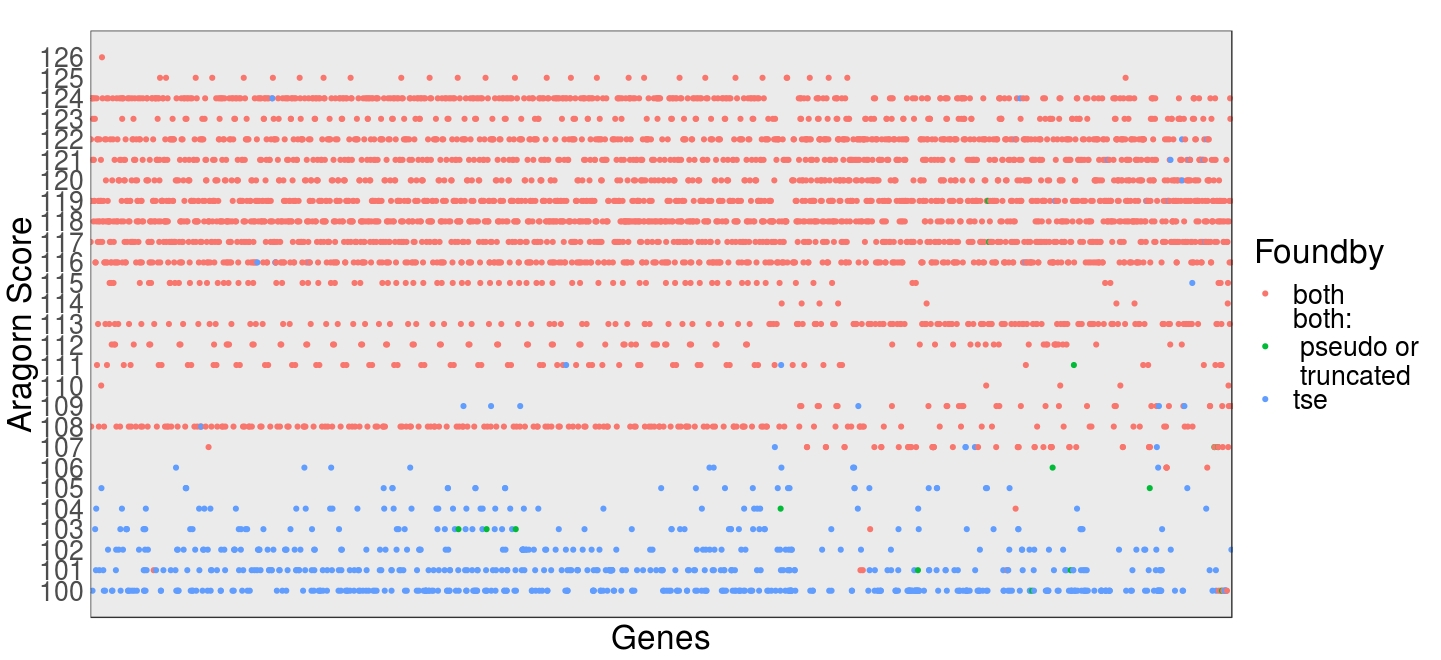
\includegraphics[width=8cm]{araScores.jpeg}}}%
    %\qquad
    \subfloat[]{{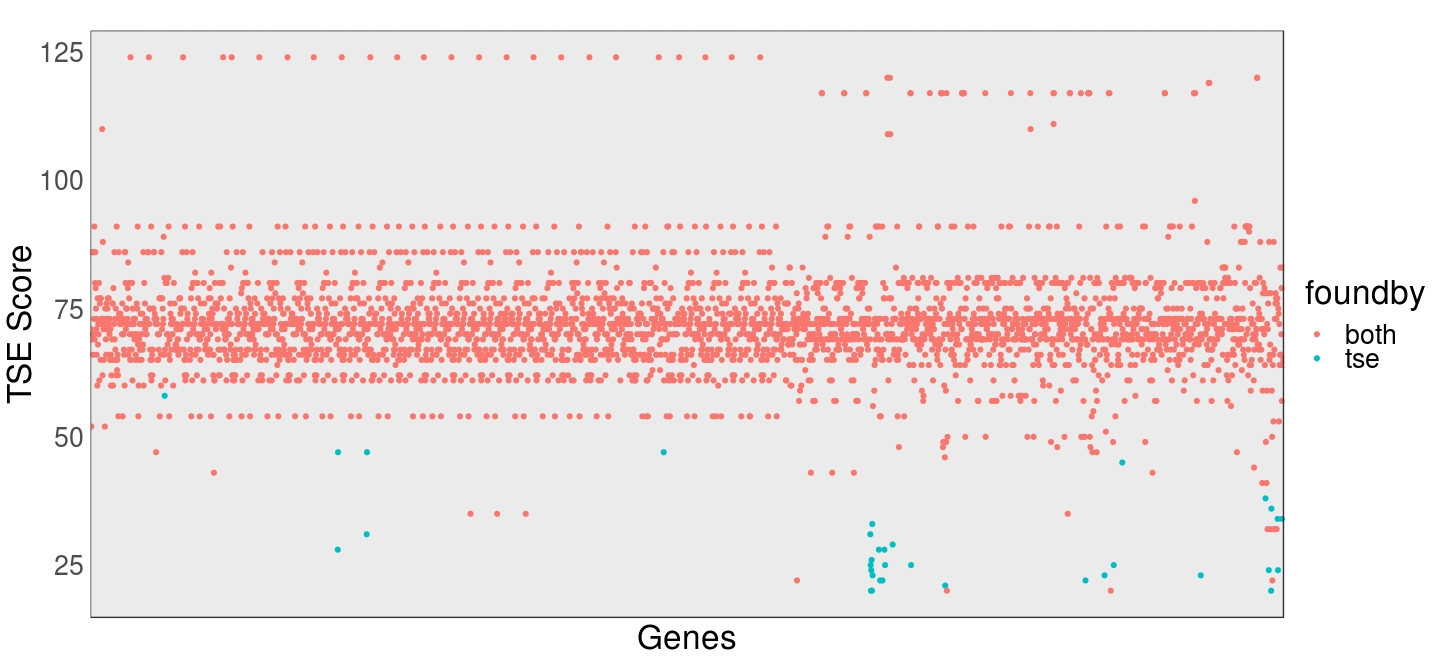
\includegraphics[width=8cm]{tseScores.jpeg}}}%
    \caption{a) ARA score of genes found by both genefinders TSE and ARA, and genes found by only ARA. b) TSE score of genes found by both genefinders and genes found by only TSE}%
    \label{fig:example}%
\end{figure}

3588 genes were left from which two genes marked as truncated by TSE were also removed. 22 genes in the remained gene set had different identity between TSE and ARA shown in table~\ref{table:2} and were partially removed.
\begin{table}[hbt]
\caption{22 genes with different anticodon assignment by two gene finders TSE and ARA}
\begin{adjustbox}{width=7cm,center}
\begin{tabular}{|c|ccc|}
\hline
tse identity|ara identity & (g|w) & (m|l) & (y|n)\\
\hline
frequency & 3 & 9 & 10\\
\hline
\end{tabular}
\label{table:2}
\end{adjustbox}
\end{table}

Each of these three ambiguties have been analysed and compared to the other genes of the same identity. Genes (y|n) were manually compare to the other identified genes with identity n and y found by both gene finders. In all cases these 10 genes were considerably more similar to the genes marked with identity Y than genes identified as N. Also, by looking at genes as clusters (a group of two or more genes found within a genome located within a thousand base pairs of each other) they were observed in clusters "LSMEM(y|n)V","V(y|n)MEMSL","LSMEMSM(y|n)V", and (y|n)V. Further we observed that there was no occurrence of genes NY or YN within any cluster, however there were 6 occurrences of YV or VY (one of them in cluster EMYV). Genes with ambiguty (m|l) were disregarded as they all appear as singleton genes, and not in any of the clusters. Genes with ambiguity (g|w) have also been removed since we were not able to resolve the ambiguity.

% summery of final genes 
The final gene set has 3574 genes from which 36 genes are found only by aragorn and the rest are predicted by both gene finders. %Table  ~\ref{table:2} shows a summary of these genes as three sets of Intersection, Union and Ara only genes.

 

% visualization of clusters of genes left:


%nucleotide composition for the TriTryp genomes is reported in Table 3.
\begin{table}[htbp]
\caption{nucleotide composition of 46 TriTryp genomes}
\begin{adjustbox}{center}
%\centering
% make it as two table
\begin{tabular}{|l|cccccccc|}\hline\hline
organism&A\%&T\%&C\%&G\%&AT\%&GC\%&Seq\#&Gene\#\\
\hline
TbruceigambienseDAL972&26&26&24&24&53&47&11&63\\
TevansiSTIB805&27&27&23&23&53&47&13&66\\
CfasciculataCfCl&21&22&29&28&43&57&31&105\\
TbruceiLister427&26&26&22&23&51&45&32&66\\
LpanamensisMHOMPA94PSC1&21&21&28&28&41&56&35&74\\
LdonovaniBHU1220&19&20&29&29&39&57&36&84\\
LdonovaniBPK282A1&19&20&29&29&39&57&36&85\\
LinfantumJPCM5&20&20&30&30&40&60&36&84\\
LmajorFriedlin&20&20&30&30&40&60&36&84\\
LmajorSD75.1&20&20&30&30&40&59&36&82\\
TcruziCLBrenerEsmeraldo-like&20&20&20&20&39&40&41&57\\
TcruziCLBrenerNon-Esmeraldo-like&21&21&22&22&42&43&41&57\\
TcruziSylvioX10-1&24&23&25&25&47&50&47&66\\
LpyrrhocorisH10&21&22&28&28&43&56&60&104\\
TbruceiTREU927&27&27&23&23&54&45&131&72\\
LbraziliensisMHOMBR75M2904&21&21&29&29&42&58&139&83\\
LgerbilliLEM452&20&20&30&29&40&59&142&81\\
LaethiopicaL147&19&20&30&29&39&59&160&83\\
LtropicaL590&19&19&29&28&38&57&160&87\\
LarabicaLEM1108&20&20&29&29&40&58&168&85\\
LturanicaLEM423&19&20&30&29&39&59&219&86\\
LspMARLEM2494&20&20&30&29&40&59&251&80\\
TtheileriEdinburgh&26&26&17&17&52&35&253&155\\
LenriettiiLEM3045&20&20&29&29&40&59&495&82\\
BayalaiB08-376&22&22&27&27&45&55&546&69\\
LmexicanaMHOMGT2001U1103&20&20&30&30&40&60&588&84\\
LbraziliensisMHOMBR75M2903&19&20&27&27&39&53&745&86\\
LmajorLV39c5&20&20&29&29&40&59&809&84\\
LpanamensisMHOMCOL81L13&21&21&29&28&42&57&856&88\\
TcruzicruziDm28c&24&24&26&26&48&52&1029&95\\
TcruziDm28c&25&25&26&25&49&50&1210&50\\
LseymouriATCC30220&22&22&28&28&44&55&1222&94\\
LtarentolaeParrotTarII&21&21&27&27&42&55&1351&78\\
EmonterogeiiLV88&23&23&26&26&46&52&1961&103\\
PconfusumCUL13&18&18&28&28&35&57&2188&61\\
LamazonensisMHOMBR71973M2269&20&20&30&30&41&59&2627&65\\
TcongolenseIL3000&21&21&20&20&43&40&2839&67\\
TgrayiANR4&23&23&27&27&46&54&2871&94\\
TrangeliSC58&24&23&27&26&47&53&7433&6\\
TvivaxY486&21&21&23&23&42&46&8290&79\\
TcruziJRcl4&24&23&26&24&47&50&15312&69\\
TcruziEsmeraldo&23&22&24&23&45&47&15803&74\\
TcruzimarinkelleiB7&22&22&23&23&43&45&16783&56\\
TcruziSylvioX10-1-2012&24&24&26&26&49&51&27019&68\\
TcruziCLBrener&23&23&27&27&47&53&29407&14\\
TcruziTulacl2&22&21&23&23&43&46&45711&119\\  \hline\hline
\end{tabular}
\label{table:3}
\end{adjustbox}
\end{table}


\begin{figure}[H]
\centering 
\tcbox[sharp corners, boxsep=1mm, boxrule=0.3mm,colback=white]{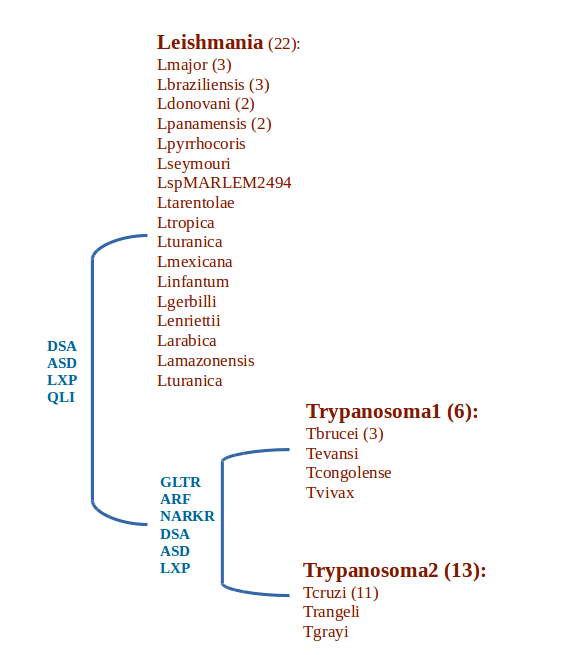
\includegraphics[scale = 0.5]{Genomeclusters.png}}
\caption[]{TriTryp genomes clustered into three classes of Leishmania(L), Trypanosoma1(T1), and Trypanosoma2(T2)}
\label{fig:Flogo} 
\end{figure}

\begin{figure}[H]
\centering 
\tcbox[sharp corners, boxsep=1mm, boxrule=0.3mm,colback=white]{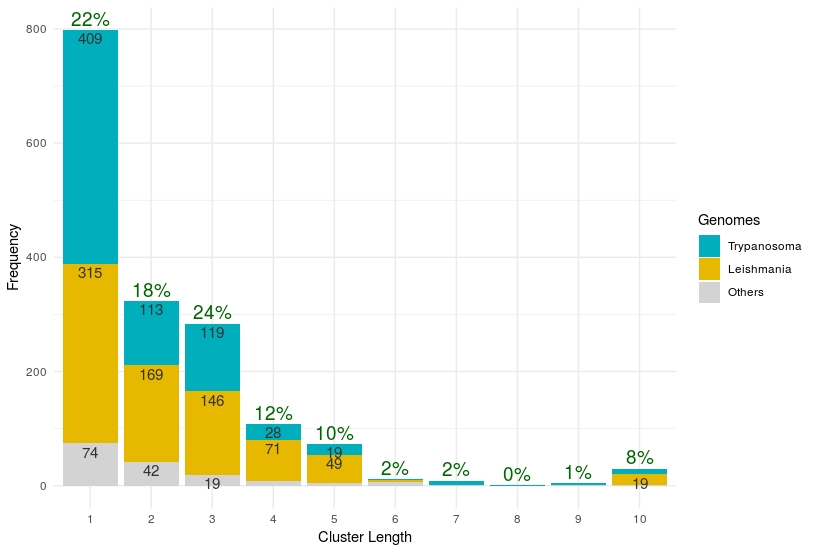
\includegraphics[width=\columnwidth]{clustSizedist.jpeg}}
\caption[]{Cluster size distribution for three categories of TryTryp genomes. Labels in green on top of each bar show the percentage of total number of genes as cluster of a specific length. Each color refers to one category of TriTryp genomes. Numbers within each color section of the bar shows the counts of clusters with a specific length.}
\label{fig:Flogo} 
\end{figure}

\begin{table}[htbp]
\caption{frequecty of gene clusters of length > 3 with frequency of atleast 2. T\% and L\% refer to the percentage of Trypanosoma and Leishmania genomes, in order, that contain the cluster}
\begin{adjustbox}{center}
\begin{tabular}{|c||c|} \hline
%%%%%% Title row starts here
Trypanosoma & Leishmania \\ \hline\hline
\begin{tabular}{l ccc}
%\hline
Cluster&dir& T\%&L\%\\
EVRH&--++&91&0\\
IVQRLTRKGW&+-----++-+&82&0\\
VIMLS&-++-+&82&0\\
CLXP&+--+&73&0\\
NYTPN&---++&64&0\\
GTGP&+--+&55&0\\
NPTYN&--+++&36&0\\
YTTY&--++&36&0\\
PGTTG&-++--&18&0\\
SLMIV&-+--+&14&0\\
EARR&--++&9&0\\
YTTT&---+&9&0\\
%\hline
\end{tabular} &

\begin{tabular}{l ccc}
%\hline
Cluster&dir& L\%&T\%\\
NARKR&+-+++&55&0\\
IQVKGLTRKR&-++++--++-&35&0\\
GLTR&++-+&30&0\\
EMSV&-+-+&20&0\\
IQVK&-+++&20&0\\
ILQQI&+--++&15&0\\
LSMEMYV&-+-++-+&15&0\\
RKRTLGKVQI&+--++----+&15&0\\
LSMEMYV&-+--+-+&10&0\\
%\hline
\end{tabular} \\ \hline
\end{tabular}
\end{adjustbox}
\end{table}





%%%%%%%%%%%%%%%%
\begin{table}[htbp]
\caption{frequecty of gene clusters of length > 2. T\% and L\% refer to the percentage of Trypanosoma and Leishmania genomes, in order, that contain the cluster}
\begin{adjustbox}{totalheight=\textheight,center}
%\scalebox{0.9}{
\begin{tabular}{|c||c|} \hline
%%%%%% Title row starts here
Trypanosoma (20 genomes) & Leishmania (22 genomes)\\ \hline\hline
\begin{tabular}{l ccc}
%\hline
Cluster&dir& T\%&L\%\\
DSA&-++&95&55\\
EVRH&--++&91&0\\
PVK&+++&91&0\\
QLI&+-+&86&0\\
RRA&--+&86&0\\
IVQRLTRKGW&+-----++-+&82&0\\
VIMLS&-++-+&82&0\\
CLXP&+--+&73&0\\
VHF&++-&68&0\\
NYTPN&---++&64&0\\
KGN&+--&59&0\\
GTGP&+--+&55&0\\
LAG&-++&45&0\\
NPTYN&--+++&36&0\\
YTTY&--++&36&0\\
GAL&--+&27&0\\
LXP&--+&23&30\\
PGTTG&-++--&18&0\\
SLMIV&-+--+&14&0\\
EARR&--++&9&0\\
KVP&---&9&0\\
MRR&-++&9&0\\
TGP&--+&9&0\\
YTTT&---+&9&0\\
ARR&-++&5&0\\
ASD&--+&5&30\\
DEDE&+-+-&5&0\\
DRTY&++++&5&0\\
EFHV&-+--&5&0\\
FHVRH&+--++&5&0\\
GEE&+--&5&0\\
GKWRTL&-+--++&5&0\\
GTGP&++-+&5&0\\
GTGPVK&+--+++&5&0\\
GTP&+-+&5&0\\
HRE&--+&5&0\\
ILIQ&-++-&5&0\\
IVQRLTKGW&+-----+-+&5&0\\
IVQRLTRWKG&+-----++-+&5&0\\
LAA&-++&5&0\\
NGK&++-&5&0\\
PTG&---&5&0\\
PXLC&-++-&5&0\\
QILI&+--+&5&0\\
QLQ&-+-&5&0\\
QVI&++-&5&0\\
RQVI&+++-&5&0\\
VHFE&++-+&5&0\\
VYIML&-+++-&5&0\\
VYIMLS&-+++-+&5&0\\
WGKRTL&-+--++&5&0\\
YTRD&----&5&0\\
YTY&--+&5&0\\
%\hline
\end{tabular} &

\begin{tabular}{l ccc}
%\hline
Cluster&dir& L\%&T\%\\
DSA&-++&55&95\\
NARKR&+-+++&55&0\\
ARF&--+&50&0\\
IQL&-++&35&0\\
IQVKGLTRKR&-++++--++-&35&0\\
PTN&-++&35&0\\
ASD&--+&30&5\\
GLTR&++-+&30&0\\
LQI&--+&30&0\\
LXP&--+&30&23\\
PXL&-++&30&0\\
VEF&-++&30&0\\
FRA&-++&25&0\\
HEF&+++&25&0\\
LXP&+-+&25&0\\
VLM&---&25&0\\
EMSV&-+-+&20&0\\
IQVK&-+++&20&0\\
SLS&+--&20&0\\
FEV&--+&15&0\\
ILQQI&+--++&15&0\\
LSMEMYV&-+-++-+&15&0\\
RKRTLGKVQI&+--++----+&15&0\\
LSMEMYV&-+--+-+&10&0\\
NTP&--+&10&0\\
ARFARF&--+--+&5&0\\
ARKR&-+++&5&0\\
ASDD&--++&5&0\\
DSV&-++&5&0\\
EML&-++&5&0\\
EMYV&++-+&5&0\\
FIQ&---&5&0\\
FIQFIQ&------&5&0\\
ILQ&+--&5&0\\
IQI&+++&5&0\\
IQQL&--++&5&0\\
IQQLI&--++-&5&0\\
IQV&-++&5&0\\
IQVKGLTR&-++++--+&5&0\\
KGL&+++&5&0\\
KVQI&---+&5&0\\
LSM&-+-&5&0\\
LSMEMSMYV&-+-++-+-+&5&0\\
LTP&--+&5&0\\
MEM&--+&5&0\\
MEMSL&--+-+&5&0\\
MEMSL&-++-+&5&0\\
MMAP&----&5&0\\
NARK&+-++&5&0\\
NWW&+++&5&0\\
PKP&+--&5&0\\
PTYN&-+-+&5&0\\
QFIQ&----&5&0\\
QLI&-+-&5&0\\
QVK&+++&5&0\\
RHLP&++++&5&0\\
RKKK&+--+&5&0\\
RKR&---&5&0\\
RKRAN&---+-&5&0\\
RKRRA&----+&5&0\\
RKRTLGKVQ&+--++----&5&0\\
SLS&++-&5&0\\
VHEF&-+++&5&0\\
VYMEMSL&-+--+-+&5&0\\
VYMEMSL&-+-++-+&5&0\\
WWNN&----&5&0\\
%\hline
\end{tabular} \\ \hline
\end{tabular}
\end{adjustbox}
\end{table}

%%%%%%%%%%%%%%%%



\begin{table}[htbp]
\caption{frequecty of gene clusters of length > 2. T1\% and T2\% refer to the percentage of Trypanosoma1 and Trypanosoma2 genomes, in order, that contain the cluster}
\begin{adjustbox}{center}
%\scalebox{0.9}{
\begin{tabular}{|c||c|} \hline
%%%%%% Title row starts here
Trypanosoma1 (6 genomes) & Trypanosoma2 (13 genomes) \\ \hline\hline
\begin{tabular}{l ccc}
%\hline
Cluster&dir& T1\%&T2\%\\
ARF&--+&83&38\\
DSA&-++&83&46\\
GLTR&++-+&83&8\\
HEF&+++&83&0\\
LXP&+-+&83&0\\
NARKR&+-+++&83&46\\
VLM&---&83&0\\
ASD&--+&67&15\\
EMSV&-+-+&67&0\\
IQVK&-+++&67&0\\
SLS&+--&67&0\\
ILQQI&+--++&50&0\\
EML&-++&17&0\\
FIQ&---&17&0\\
FIQFIQ&------&17&0\\
ILQ&+--&17&0\\
IQI&+++&17&0\\
IQV&-++&17&0\\
KGL&+++&17&0\\
LXP&--+&17&38\\
QFIQ&----&17&0\\
QLI&-+-&17&0\\
QVK&+++&17&0\\
RHLP&++++&17&0\\
SLS&++-&17&0\\
%\hline
\end{tabular} &

\begin{tabular}{l ccc}
%\hline
Cluster&dir& T1\%&T2\%\\
IQL&-++&54&0\\
IQVKGLTRKR&-++++--++-&54&0\\
PTN&-++&54&0\\
DSA&-++&46&83\\
LQI&--+&46&0\\
NARKR&+-+++&46&83\\
VEF&-++&46&0\\
ARF&--+&38&83\\
LXP&--+&38&17\\
PXL&-++&38&0\\
FRA&-++&31&0\\
FEV&--+&23&0\\
LSMEMYV&-+-++-+&23&0\\
RKRTLGKVQI&+--++----+&23&0\\
ASD&--+&15&67\\
LSMEMYV&-+--+-+&15&0\\
NTP&--+&15&0\\
ARFARF&--+--+&8&0\\
ASDD&--++&8&0\\
DSV&-++&8&0\\
EMYV&++-+&8&0\\
GLTR&++-+&8&83\\
IQQLI&--++-&8&0\\
IQVKGLTR&-++++--+&8&0\\
LSM&-+-&8&0\\
LSMEMSMYV&-+-++-+-+&8&0\\
MEM&--+&8&0\\
MEMSL&--+-+&8&0\\
MMAP&----&8&0\\
NARK&+-++&8&0\\
PTYN&-+-+&8&0\\
RKKK&+--+&8&0\\
RKR&---&8&0\\
RKRAN&---+-&8&0\\
RKRRA&----+&8&0\\
RKRTLGKVQ&+--++----&8&0\\
VYMEMSL&-+--+-+&8&0\\
VYMEMSL&-+-++-+&8&0\\
WWNN&----&8&0\\
%\hline
\end{tabular} \\ \hline
\end{tabular}
\end{adjustbox}
\end{table}



\begin{table}[htbp]
\caption{Sets of clusters with potential variations (duplication,deletion,inversion). There are three genome classes T, L and O which refer to Trypanosoma, Leishmania and Other genomes in order. }
\begin{adjustbox}{totalheight=\textheight,center}
\begin{tabular}{|c||c|} \hline
%%%%%% Title row starts here
\begin{tabular}{l ccccc}
%\hline
clusters&set&Genomeclass&Tdirs&Ldirs&Odirs\\
\rowcolor{shadecolor}
GEE&0&L&&-++&\\
LAA&0&L&&+-+-&\\
MEM&0&L&&++++&\\
PKP&0&L&&--++&\\
RKKK&0&L&&-+--&\\
YTY&0&L&&+--++&\\
III&0&LT&--+&--+&\\
LSSS&0&O&&&+++\\
QLQ&0&O&&&--+-+\\
WWNN&0&O&&&--++-+\\
KKN&0&OL&&+--+&+--+\\
YTTT&0&OL&&--++&--++\\
MRR&0&OLT&-++&-++&-++\\
ARR&0&T&--+&&\\
DEDE&0&T&--+--+&&\\
GAA&0&T&-+++&&\\
IQI&0&T&--++&&\\
NWW&0&T&-++&&\\
RKR&0&T&-++&&\\
RRA&0&T&-+-+&&\\
SLS&0&T&++-+&&\\
YTTY&0&T&--+&&\\
%\rowcolor{Gainsboro}
\rowcolor{lightgray}
ARF&1&T&---&&\\
ARFARF&1&T&------&&\\
FRA&1&T&-++&&\\
\rowcolor{shadecolor}
ENKRRA&2&L&&--+&\\
NARK&2&L&&+--&\\
NARKR&2&L&&-+--++&\\
RKRAN&2&L&&+--+|++-+&\\
RKRRA&2&L&&+--+++&\\
RRAE&2&L&&+-+&\\
ARKR&2&O&&&+--\\
EARR&2&O&&&---\\
RKAREN&2&T&++-+&&\\
\rowcolor{lightgray}
ASDD&3&L&&--+&\\
DSA&3&O&&&--+\\
ASD&3&T&+++&&\\
\rowcolor{shadecolor}
CLXP&4&L&&-++-&\\
LXC&4&T&+--&&\\
LXP&4&T&+--++&&\\
LXPXP&4&T&+++&&\\
PXL&4&T&-++&&\\
PXLC&4&T&--++&&\\
\rowcolor{lightgray}
DNE&5&T&--++-&&\\
\rowcolor{shadecolor}
DRTY&6&T&-++&&\\
YTRD&6&T&-+++&&\\
\rowcolor{lightgray}
DSV&7&T&-++++--+&&\\
\rowcolor{shadecolor}
HEF&9&L&&+-----+-+&\\
VEF&9&L&&+-----++-+&\\
EFHV&9&O&&&--++++-+-\\
FEV&9&O&&&+--\\
VHEF&9&OL&&+-----++-+&+---+-+-++\\
VHFE&9&OL&&+--&+--\\
EFFVH&9&T&-++++--++-&&\\
VHF&9&T&+++&&\\
\rowcolor{lightgray}
EMYV&10&L&&---&\\
LSMEMSMYV&10&L&&-++&\\
LSMEMYV&10&L&&-++&\\
EML&10&O&&&++-\\
EMSV&10&O&&&--++\\
VIMLS&10&O&&&-+---+\\
VLM&10&O&&&----\\
VYIMLS&10&O&&&--++-+\\
VYMEMSL&10&O&&&---\\
LSM&10&T&---+&&\\
LSMIVY&10&T&--+&&\\
MEMSL&10&T&-+-&&\\
MEYSL&10&T&-+-++-+-+&&\\
SLMIV&10&T&-+-++-+|-+--+-+&&\\
VYIML&10&T&--+&&\\
%\hline
\end{tabular} &

\begin{tabular}{l ccccc}
%\hline
clusters&set&Genomeclass&Tdirs&Ldirs&Odirs\\
\rowcolor{shadecolor}
EVRH&13&LT&+-+|--+&--+&\\
HRE&13&O&&&--+-+\\
RVHE&13&T&--+&&\\
\rowcolor{lightgray}
FHVRH&14&T&--+-+|-++-+&&\\
\rowcolor{shadecolor}
QFIQ&15&L&&-++&\\
FIQ&15&O&&&----+\\
FIQFIQ&15&T&----&&\\
\rowcolor{lightgray}
FSI&16&T&+-++&&\\
\rowcolor{shadecolor}
KLAG&17&L&&++-&\\
LAG&17&L&&--+++&\\
GAL&17&T&+-+++&&\\
\rowcolor{lightgray}
ILQ&18&L&&-++--&\\
IQL&18&L&&---&\\
IQVKGLTR&18&L&&-++-&\\
IVQRLTKGW&18&L&&-+-&\\
IVQRLTRWKG&18&L&&++-&\\
RKRTLGKVQI&18&L&&+++-&\\
IVQRLTRKGW&18&O&&&+++\\
LQI&18&O&&&---++-\\
VGWRTQI&18&O&&&--++\\
WGKRTL&18&O&&&-++-\\
ILIQ&18&OL&&---++&---++\\
IQV&18&OL&&+++&+++\\
ITRLQVGWR&18&OL&&+--+&+--+\\
RQVI&18&OL&&--+&--+\\
IVQ&18&OLT&-+-&+-+&+-+\\
GKWRTL&18&T&--+&&\\
GLTR&18&T&+++&&\\
ILQQI&18&T&+--&&\\
IQQL&18&T&-++&&\\
IQQLI&18&T&-+-+&&\\
IQVK&18&T&-++&&\\
IQVKGLTRKR&18&T&----&&\\
KGL&18&T&+++&&\\
KVQI&18&T&++++&&\\
LTRKGW&18&T&+--+&&\\
QILI&18&T&---&&\\
QLI&18&T&---+-&&\\
QVI&18&T&----+&&\\
QVK&18&T&+--++----&&\\
RKRTLGKVQ&18&T&+--++----+&&\\
\rowcolor{shadecolor}
GTGP&19&L&&-+--+&\\
TGP&19&L&&++-+&\\
PGTTG&19&O&&&+-+-+--\\
GTP&19&OL&&--+&--+\\
PVK&19&OL&&++-&+++\\
GTGPVK&19&T&+--|++-&&\\
KVP&19&T&-++&&\\
PTG&19&T&-+++&&\\
\rowcolor{lightgray}
KGN&22&L&&-++-+&\\
NGK&22&T&---&&\\
\rowcolor{shadecolor}
LTP&24&L&&-+++-&\\
\rowcolor{lightgray}
MMAP&25&OL&&-+++-+&-+++-+\\
\rowcolor{shadecolor}
NTP&26&L&&-+--++&\\
YTN&26&L&&---+&\\
PTN&26&O&&&---\\
PTYN&26&OL&&----&----\\
NPTYN&26&T&-+-++-+|-+--+-+&&\\
NYTPN&26&T&----&&\\
\rowcolor{shadecolor}
QPL&27&L&&--++&\\
\rowcolor{shadecolor}
RHLP&28&L&&--+&\\
%\hline
\end{tabular} \\ \hline
\end{tabular}
\end{adjustbox}
\end{table}



%----------------------------------------------------------------------------------------
%	BIBLIOGRAPHYyour own dat
%----------------------------------------------------------------------------------------
\
\renewcommand{\refname}{\spacedlowsmallcaps{References}} % For modifying the bibliography heading

\bibliographystyle{unsrt}

\bibliography{sample.bib} % The file containing the bibliography

%----------------------------------------------------------------------------------------

\end{document}
